\chapter{Selective sequencing}

\label{kap:selSeq} % id kapitoly pre prikaz ref

In this chapter, we are going to look at what is selective sequencing. What are the
advantages that this method brings, the main challenges in this area and current state
of research in this area.

\section{DNA sequencing}

One of the biggest goals of bioinformatics is to obtain DNA sequence (sequence of A, C, G, T)
from some biological sample. One of the devices that serve this purpose is MinION\cite{lu2016oxford}.
MinION is a small, cheap and versatile DNA sequencer. One drawback of the MinION is
that it does not produce a nucleotide sequence directly. Instead, it produces a signal.
Idea is that as the biological string of DNA is passing through the pore of MinION,
we can observe changes in the flow of an electric current passing through the pore.
This electric current called signal is measured over discrete time. Example, how
this signal could look is on the figure \ref{obr:minIonCurrent}.

\begin{figure}
\centerline{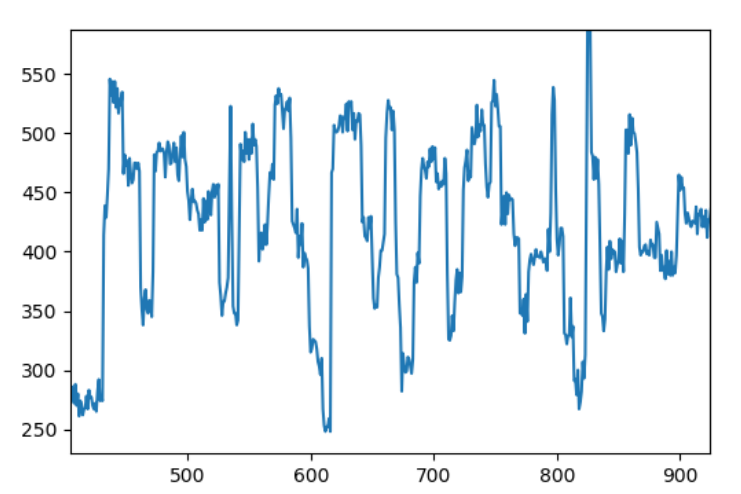
\includegraphics[width=0.7\textwidth, height=0.3\textheight]{images/signal}}
\caption[MinION signal]{Electric current (signal) coming from MinION.}
%id obrazku, pomocou ktoreho sa budeme na obrazok odvolavat
\label{obr:minIonCurrent}
\end{figure}

It's not yet clear how we obtain DNA sequence from this signal. As the string of DNA
is passing through the pore, only a small number of nucleotides in the proximity of pore
shape the output signal. So from the signal, using a method called base-calling, we
can tell how the string of DNA looked like based on the measurements of signal
throughout the time. Despite big improvements in the base-calling algorithms, the overall
process of base-calling is quite slow and resource-intensive.

\section{Selective sequencing}

\subsection{Idea}

MinION has one special ability that helps us in certain scenarios. It can reject
DNA string that is currently passing through the pore. It effectively reverses
the string’s direction and throws it away. Selective sequencing is the idea that
based on the incoming signal, we can tell if we are interested in sequencing current
DNA string and can decide if we want to continue or reject this string. This happens
on-the-fly so we need to make the decision until the end of the current read. This means
we don't have time to turn our signal into a nucleotide sequence as the reads are
quite short in this sense. This is a reason why we have to work with a raw signal.

\subsection{Usage}

What are the benefits of selective sequencing? In case we are not interested
in some DNA that we know is contained in our sample, we can use this technique to
reject unwanted DNA string. Why would we do that in the first place? Obtaining
nucleotide sequence from the signal is in some scenarios unnecessary and too
costly process in terms of performance. 

Let's say we are trying to find an exact type of virus in human blood. We can
reject all human DNA samples because we are not interested in processing human
DNA. We could also filter in a positive way. So we could say, that we are only
interested in sequencing DNA that produces a signal in some sense similar to our
chosen sample. This all means saving a lot of time and computing power in certain
cases, for example during the diagnosis process.

What are some drawbacks of selective sequencing? In order to find out if the currently
passing string is from human DNA, we have to have some human signal beforehand.
This is of course in some sense limiting factor as we need a sample signal from
the species that we want to filter. The other problem is that in the case of misclassifying
some signal as not interesting, we lost information about the corresponding
read.

\section{Current state of selective sequencing}
